\documentclass[12pt,letterpaper]{article}

\usepackage[bookmarks=true]{hyperref}
\usepackage{graphicx}
\usepackage{geometry}
\usepackage{fontspec}
\usepackage{xunicode}
\usepackage{xltxtra}
\usepackage{color,colortbl}
\usepackage{url}
\usepackage[table]{xcolor}
\usepackage{multirow}
\usepackage{xtab}
\usepackage[final]{pdfpages}
\usepackage{subfigure}
\usepackage{amsmath,amssymb}


\definecolor{Gray}{gray}{0.9}

\defaultfontfeatures{Mapping=tex-text} % converts LaTeX specials (``quotes'' --- dashes etc.) to unicode

\setromanfont [Ligatures={Common}]{Cardo}
\setmonofont{Inconsolata}

% Set your name here
\def\name{Patrick J. Martin}

% Replace this with a link to your CV if you like, or set it empty
% (as in \def\footerlink{}) to remove the link in the footer:
\def\footerlink{}

% The following metadata will show up in the PDF properties
\definecolor{darkblue}{rgb}{0.0,0.0,0.5}
\hypersetup{
  colorlinks = true,
  linkcolor=darkblue,
  urlcolor = darkblue,
  pdfauthor = {\name},
  pdftitle = {\name: PJM Udacity Capstone Report},
  pdfpagemode = UseNone
}

\geometry{
  body={6.5in, 8.5in},
  left=1.0in,
  top=1.0in,
  bottom=1.0in
}

\subfigcapmargin = .5cm

% Customize page headers
\pagestyle{myheadings}
\markright{\name}
\thispagestyle{empty}

% Custom section fonts
\usepackage{sectsty}
\sectionfont{\rmfamily\mdseries\Large}
\subsectionfont{\rmfamily\mdseries\large}

% Don't indent paragraphs.
\setlength\parindent{0em}

% Make lists without bullets
\renewenvironment{itemize}{
  \begin{list}{}{
    \setlength{\leftmargin}{1.5em}
  }
}{
  \end{list}
}

% courtesy D. Hovemeyer
\newenvironment{denseItemize}{%
\begin{list}{}{\setlength{\itemsep}{0.4em}\setlength{\leftmargin}{1.5em}\setlength{\parsep}{0in}}}{\end{list}}
%\setlength{\topsep}{.1mm}

\begin{document}

\pagestyle{myheadings}
\markright{\name---Capstone Project}
\thispagestyle{empty}

%{\LARGE \name} \\
%\smallskip
%\smallskip
{\Large Deep Learning Applied to Digit Sequence Classification} \\ 

\smallskip

Patrick Martin \\
Udacity MLND Capstone Report \\
\rule{\columnwidth}{1pt}


\subsection*{Introduction}










\subsection*{SVHN Data Exploration}

To train and test my digit sequence classifier, I used the street view house numbers data set \cite{SVHNData}.
This data set is available in two forms: full numbers with bounding boxes and cropped $32\times32$ pixel images.
I chose the full number data set and pre-processed the images by loading the bounding box meta data held within the \verb|digitStruct.mat| file. \\

My preprocessing algorithm iterated over the entire training and testing data and performed the following operations on each \verb|digitStruct| object:
\begin{enumerate}

	\item Extracted the image and label data, which are used as the inputs and labels for the deep neural network model.
	\item Computed a crop boundary by moving the top-left corner by 10\% toward the axis origin. I computed the bottom-right edge by adding 15\% over the width and 5\% in the height. This cropped image was then resized to a $32\times32$ pixel image.
	\item Computed the \emph{one-hot encoding} vectors of the labels. The encoded labels are represented with a 2D array of dimension $6\times10$, where the row dimension indicates 1) the length of the sequence and 2) the digits in up to five places. The column dimension of 10 represents a one-hot encoding of a value between 0 and 10. The values 0-9 represent digits and 10 represents the lack of a digit.
\end{enumerate}

\begin{figure*}[ht]
    \centering
    \subfigure[Original image of ``50''.]{
        \centering
        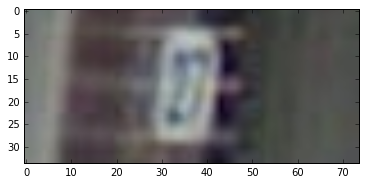
\includegraphics[width=0.33\textwidth]{graphics/train/image1.png}
    }
    \subfigure[Original image of ``25''.]{
        \centering
        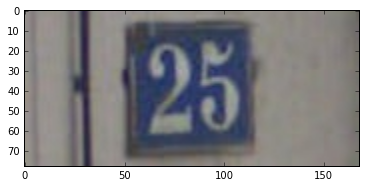
\includegraphics[width=0.33\textwidth]{graphics/train/image2.png}
    }
    \subfigure[Original image of ``115''.]{
        \centering
        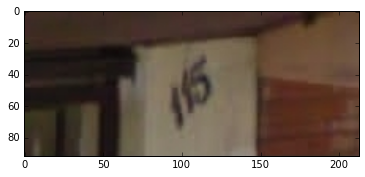
\includegraphics[width=0.33\textwidth]{graphics/train/image3.png}
    }
    \subfigure[Original image of ``60''.]{
        \centering
        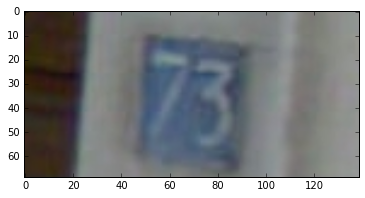
\includegraphics[width=0.33\textwidth]{graphics/train/image4.png}
    }
    \caption{An illustration of four randomly sampled images from the training data set. These images are passed into Step 2 of my preprocessing algorithm.}
    \label{fig:trainingpics}
\end{figure*}


\begin{figure*}[ht]
    \centering
    \subfigure[``50'']{
        \centering
        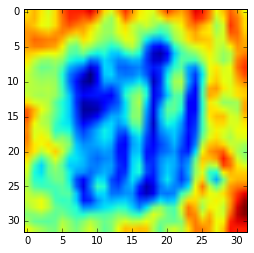
\includegraphics[width=0.2\textwidth]{graphics/train/image1_crop.png}
    }
    \subfigure[``25'']{
        \centering
        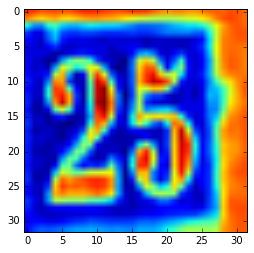
\includegraphics[width=0.2\textwidth]{graphics/train/image2_crop.png}
    }
    \subfigure[``115'']{
        \centering
        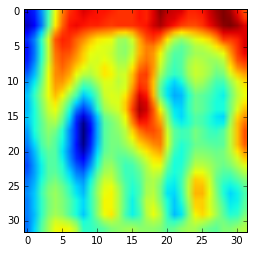
\includegraphics[width=0.2\textwidth]{graphics/train/image3_crop.png}
    }
    \subfigure[``60'']{
        \centering
        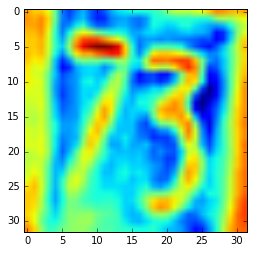
\includegraphics[width=0.2\textwidth]{graphics/train/image4_crop.png}
    }
    \caption{The processed images from Figure \ref{fig:trainingpics}, which were converted to grayscale, cropped to a square shape, and resized to a $32\times32$ pixel image.}
    \label{fig:trainingpics_cropped}
\end{figure*}

\begin{figure*}[ht]
    \centering
    \subfigure[Encoding for ``50''.]{
        \centering
        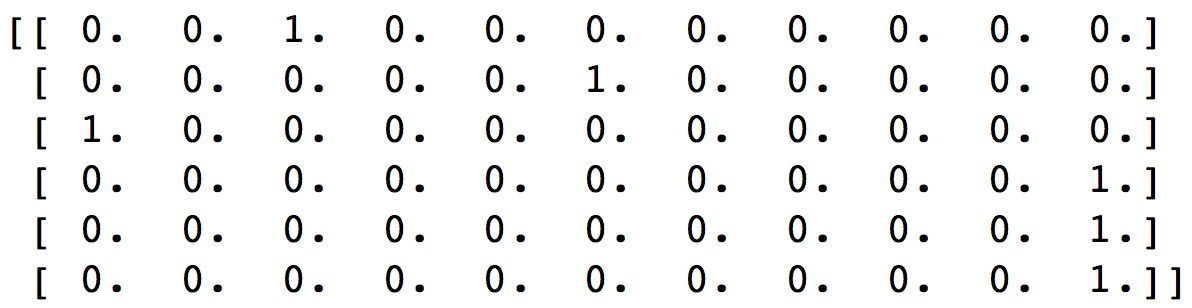
\includegraphics[width=0.45\textwidth]{graphics/train/image1_onehot.png}
    }
    \subfigure[Encoding for ``25''.]{
        \centering
        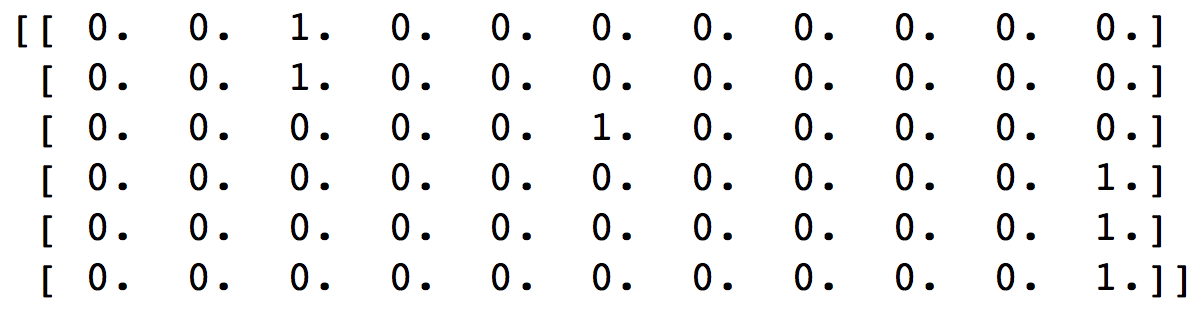
\includegraphics[width=0.45\textwidth]{graphics/train/image2_onehot.png}
    }
    \caption{This figure shows the one-hot encoding for two of the example training images. Since each of these digit sequences has length 2, rows indices 3 through 5 have an encoding of 10, which means there is no digit in positions 3, 4, or 5.}
    \label{fig:training_onehot}
\end{figure*}


\begin{figure*}[ht]
    \centering
    \subfigure[Original image of ``33''.]{
        \centering
        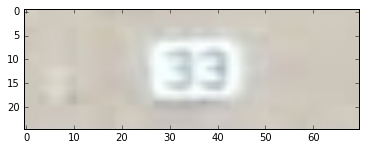
\includegraphics[width=0.33\textwidth]{graphics/test/image1.png}
    }
    \subfigure[Original image of ``299''.]{
        \centering
        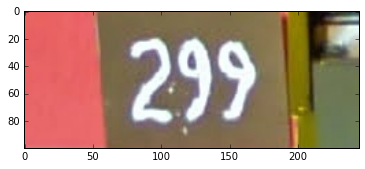
\includegraphics[width=0.33\textwidth]{graphics/test/image2.png}
    }
    \subfigure[Original image of ``128''.]{
        \centering
        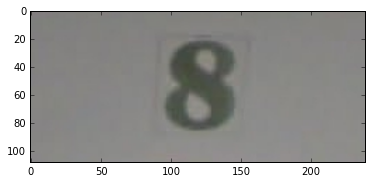
\includegraphics[width=0.33\textwidth]{graphics/test/image3.png}
    }
    \subfigure[Original image of ``50''.]{
        \centering
        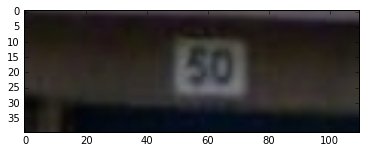
\includegraphics[width=0.33\textwidth]{graphics/test/image4.png}
    }
    \caption{The pre-processing algorithm was applied to four randomly selected test images. This figure shows their original form.}
    \label{fig:testingpics}
\end{figure*}


\begin{figure*}[ht]
    \centering
    \subfigure[``33'']{
        \centering
        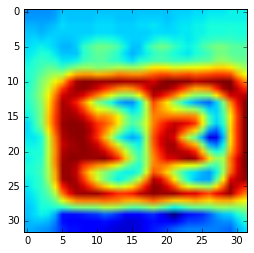
\includegraphics[width=0.2\textwidth]{graphics/test/image1_crop.png}
    }
    \subfigure[``299'']{
        \centering
        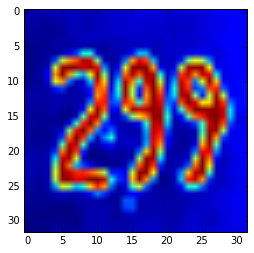
\includegraphics[width=0.2\textwidth]{graphics/test/image2_crop.png}
    }
    \subfigure[``128'']{
        \centering
        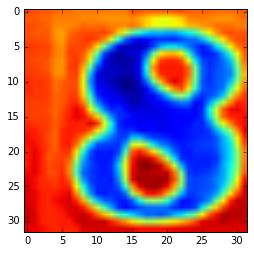
\includegraphics[width=0.2\textwidth]{graphics/test/image3_crop.png}
    }
    \subfigure[``50'']{
        \centering
        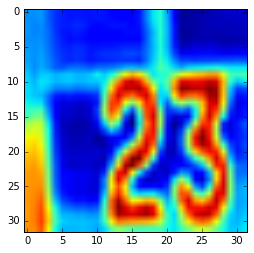
\includegraphics[width=0.2\textwidth]{graphics/test/image4_crop.png}
    }
    \caption{The processed images from Figure \ref{fig:testingpics}.}
    \label{fig:testingpics_cropped}
\end{figure*}

\begin{figure*}[ht]
    \centering
    \subfigure[Encoding for ``33''.]{
        \centering
        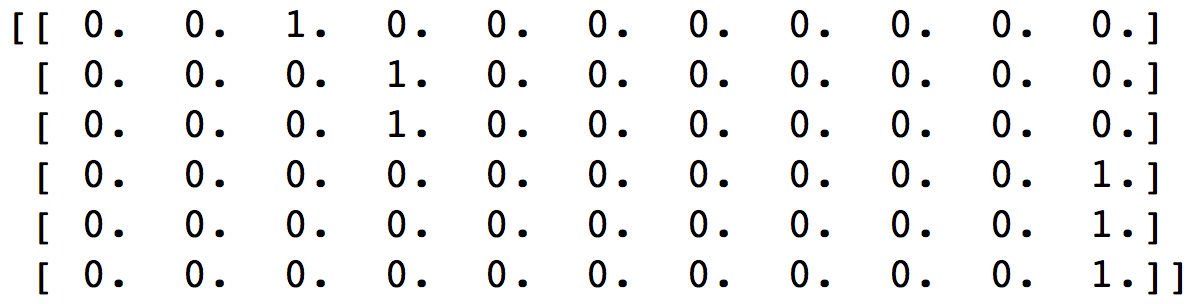
\includegraphics[width=0.45\textwidth]{graphics/test/image1_onehot.png}
    }
    \subfigure[Encoding for ``299''.]{
        \centering
        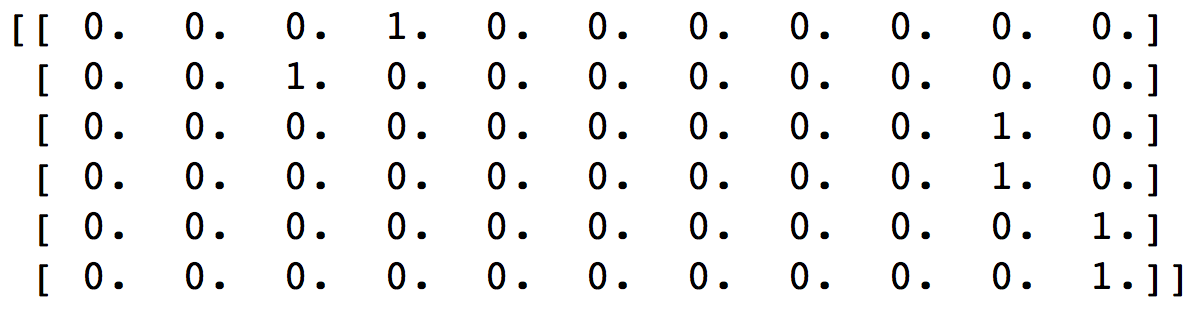
\includegraphics[width=0.45\textwidth]{graphics/test/image2_onehot.png}
    }
    \caption{This figure shows the encoding for two test images: ``33'' and ``299''.}
    \label{fig:training_onehot}
\end{figure*}


\begin{thebibliography}{99}

\bibitem{SVHNData}
http://ufldl.stanford.edu/housenumbers/

\end{thebibliography}
























\end{document}